\documentclass[sigplan]{acmart}\settopmatter{printfolios=true,printccs=false,printacmref=false}
\acmConference[PL'18]{ACM SIGPLAN Conference on Programming Languages}{January 01--03, 2018}{New York, NY, USA}
\acmYear{2018}
\acmISBN{} % \acmISBN{978-x-xxxx-xxxx-x/YY/MM}
\acmDOI{} % \acmDOI{10.1145/nnnnnnn.nnnnnnn}
\startPage{1}
\setcopyright{none}

\bibliographystyle{ACM-Reference-Format}

\begin{document}
\title{Wrattler: \textnormal{Making notebooks reproducible, live and smart}}

\author{Tomas Petricek}
\affiliation{
  \institution{The Alan Turing Institute}
  \city{London}
  \country{UK}
}
\email{tomas@tomasp.net}
\author{Charles Sutton}
\affiliation{
  \institution{University of Edinburgh}
  \city{Edinburgh}
  \country{UK}
}
\email{csutton@inf.ed.ac.uk}
\author{James Geddes}
\affiliation{
  \institution{The Alan Turing Institute}
  \city{London}
  \country{UK}
}
\email{jgeddes@turing.ac.uk}

\definecolor{cmtclr}{rgb}{0.0,0.6,0.0}
\definecolor{kvdclr}{rgb}{0.0,0.0,0.6}
\definecolor{numclr}{rgb}{0.0,0.4,0.0}
\definecolor{strclr}{rgb}{0.4,0.4,0.0}
\definecolor{rstrclr}{rgb}{0.5,0.1,0.0}
\definecolor{prepclr}{rgb}{0.6,0.0,0.2}
\newcommand{\vect}[1]{\langl #1 \rangl}
\newcommand{\langl}{\begin{picture}(4.5,7)
\put(1.1,2.5){\rotatebox{60}{\line(1,0){5.5}}}
\put(1.1,2.5){\rotatebox{300}{\line(1,0){5.5}}}
\end{picture}}
\newcommand{\rangl}{\begin{picture}(4.5,7)
\put(.9,2.5){\rotatebox{120}{\line(1,0){5.5}}}
\put(.9,2.5){\rotatebox{240}{\line(1,0){5.5}}}
\end{picture}}
\newcommand{\ball}[1]{\FPeval{\result}{clip(201+#1)}\textnormal{\ding{\result}}}
\newcommand{\lsep}{~\,|\,~}
\newcommand{\num}[1]{\textcolor{numclr}{#1}}
\newcommand{\str}[1]{\textnormal{\textcolor{strclr}{\sffamily "#1"}}}
\newcommand{\strf}[1]{\textnormal{\textcolor{strclr}{\sffamily #1}}}
\newcommand{\rstr}[1]{\textnormal{\textcolor{rstrclr}{\sffamily "#1"}}}
\newcommand{\ident}[1]{\textnormal{\sffamily #1}}
\newcommand{\qident}[1]{\textnormal{\sffamily \textquotesingle #1\textquotesingle}}
\newcommand{\dom}{\ident{dom}}
\newcommand{\kvd}[1]{\textnormal{\textcolor{kvdclr}{\sffamily #1}}}

\newcommand{\bndclr}[1]{\textcolor{kvdclr}{#1}}
\newcommand{\bkndclr}[1]{\textcolor{prepclr}{#1}}
\newcommand{\blblclr}[1]{\textcolor{numclr}{#1}}
\newcommand{\bnd}[1]{\textnormal{\textcolor{kvdclr}{\sffamily #1}}}
\newcommand{\bknd}[1]{\textnormal{\textcolor{prepclr}{\sffamily #1}}}
\newcommand{\blbl}[1]{\textnormal{\textcolor{numclr}{\sffamily #1}}}

\begin{abstract}
Notebook systems such as Jupyter became a popular programming environment for data science, because 
they support interactive data exploration and provide a convenient way of interleaving code, 
comments and visualizations. However, notebooks also suffer from reproducibility issues and make
versioning and provenance tracking difficult.

In this paper, we present Wrattler, a new notebook system with an architecture that addresses the
above issues. Wrattler stores all state in a data store and separates state management from 
script evaluation. This makes it possible to support versioning, guarantee reproducibility, track 
data provenance, but also allow richer forms of interactivity and integrate AI tools that help
automate routine data wrangling tasks.
\end{abstract}
\keywords{notebook, dependency graph, live coding, AI}
\maketitle

\section{Introduction}
Data science is an iterative, exploratory process that requires a collaboration between a computer
system and a human. Notebook systems support this interaction model by making it easy to run 
snippets of code and see results without leaving the notebook. However, typical notebook systems,
such as Jupyter suffer from a number of problems:

\paragraph{Limited reproducibility.} Cells can be executed out-of-order or modified without re-evaluating 
the notebook. This means that running all cells from scratch may give different results than those 
originally seen in the notebook.

\paragraph{Opaque state management.} All state is managed by the execution engine, or \emph{kernel}.
This makes the state invisible to tools such as version control systems and makes it hard to 
track provenance in a notebook.

\paragraph{Limited interaction.} Notebooks execute code at the granularity of an entire cell. 
This means that even simple code change may trigger a long-running computation and, as a result, 
notebooks do not always provide rapid feedback.

\paragraph{Single language.} When using a notebook, the state is managed by a single \emph{kernel}.
This makes it difficult to combine multiple programming languages in a single notebook, or build
third-party tools that would inspect the state and provide data analysts with hints about data.

\vspace{1em}
\noindent
In this paper, we present Wrattler, a new notebook system that addresses the above issues.
This is made possible by two key aspects of the Wrattler architecture (Section~\ref{sec:arch}). 

First, Wrattler maintains a dependency graph between cells and often also function calls inside
a single cell (Section~\ref{sec:comp-deps}). When a cell is changed, relevant parts of a graph
are invalidated. This guarantees reproducibility and it enables more efficient re-computation, 
because values of unaffected nodes can be reused.
Second, Wrattler separates state management from code execution (Section~\ref{sec:comp-data}). 
The \emph{data store} is responsible for managing state. It handles versioning, provenance tracking 
and enables multiple independent languages and tools to operate on the state of a notebook. 

Together, these two changes to the standard architecture of notebook systems make Wrattler notebooks
(Section~\ref{sec:results}) reproducible (with an easy and reliable state rollback), live (with 
efficient re-computation on change) polyglot and smart (allowing the integration of multiple 
execution engines and third-party AI tools). 

\begin{figure}[b]
\vspace{-1em}
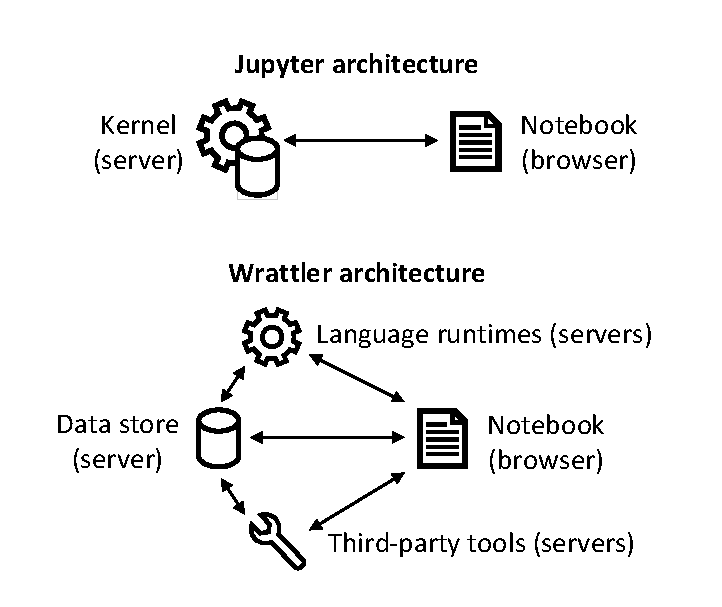
\includegraphics[scale=0.6]{diagram.pdf}
\vspace{-0.5em}
\caption{\small{In notebook systems such as Jupyter, state and execution is managed by a kernel. In
  Wrattler, those functions are split between data store and language runtimes. Data in the data store
  can be also accessed by other thrd-party tools.}}
\label{fig:arch}
\end{figure}

\section{Wrattler architecture}
\label{sec:arch}

In standard notebook systems, such as Jupyter, the state and execution is handled by a 
\emph{kernel}. The notebook running in a browser sends commands to the kernel to evaluate 
cells selected by the user. As illustrated in Figure~\ref{fig:arch}, Wrattler splits the 
server functionality between the following components:

\paragraph{Data store.} Imported external data, results of running scripts and of 
running third-party tools are stored in the data store. The data store keeps version history
and annotates data with metadata such as types, inferred semantics and provenance.

\paragraph{Language runtimes.} Code in notebook cells is evaluated by language runtimes.
The runtimes read input data from and write results back to the data store. Wrattler supports
language runtimes that run code on the server (similar to Jupyter kernels), but also language
runtimes that parse and evaluate code directly in the browser.

\paragraph{Third-party tools.} In addition to language runtimes, other tools can contribute
to data analysis by analysing data in the data store. In Wrattler, this includes AI assistants 
that help, for example, with data cleaning, type inference and data extraction from raw 
input data.

\paragraph{Notebook.} The notebook is displayed in a web browser and orchestrates 
all other components. The browser builds a dependency graph between cells or individual 
expressions in the cells. It calls language runtimes to evaluate code that has changed,
third-party tools to provide hints and reads data from the data store to display results.  

\begin{figure}
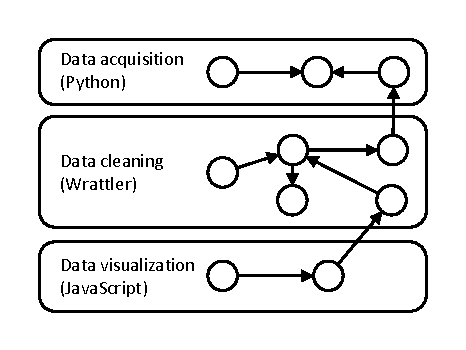
\includegraphics[scale=1,trim=0.5cm 0.5cm 0.5cm 0.5cm]{graph.pdf}
\caption{\small{Dependency graph of a sample notebook with three cells. The cells are written
in Python, Wrattler script and JavaScript. The browser builds a fine-grained dependency graph
for Wrattler script that can be parsed and analysed in the browser.}}
\label{fig:deps}
\vspace{-0.5em}
\end{figure}

\section{Wrattler components}
\label{sec:comp}

Wrattler consists of a notebook user interface running in the web browser, which communicates 
with a number of server-side components including language runtimes, the data store and third-party 
tools. In this section, we discuss the components in more detail.

\subsection{TheGamma script}
\label{sec:comp-gamma}

The Wrattler architecture supports languages that require running a separate language runtime
as a server, but also languages that can be fully evaluated in the browser. To illustrate this
feature, we integrated Wrattler with TheGamma [X], a simple browser-based language for data
exploration.

As an example, we use a data set with broadband speed published by the UK government [X].
The following TheGamma script loads the raw CSV file, groups rows by whether they represent
rural or urban area and then calculates average download speed for both of the kinds of areas:
%
\begin{equation*}
\begin{array}{l}
\ident{web.loadTable}(\str{https://.../bb2014.csv}).\ident{explore}.\\
\quad\qident{group data}.\qident{by Urban/rural}.\\
\qquad\qident{average Download speed (Mbit/s) 24 hrs}  
\end{array}
\end{equation*}
%
Here, identifiers such as \qident{by Urban/rural} are generated by a \emph{type provider} [X] 
and the user typically interacts by selecting one of generated members through an auto-complete
(hence the long explicity names are acceptable). For the purpose of this paper, the most 
important aspect is that TheGamma scripts can be parsed, checked and evaluated in the browser.

\subsection{Dependency graph}
\label{sec:comp-deps}

When opening a notebook, Wrattler parses the source of the notebook (consisting of text cells and
code cells) and constructs a dependency graph, which serves as a runtime representation of the
notebook. 

As an example, consider a simpler notebook with three cells. The first cell, written in Python,
downloads data and exports the result as a data frame; the second cell is written in TheGamma script
and performs data cleaning and the third cell creates a visualization in JavaScript. The
resulting dependency graph is shown in Figure~\ref{fig:deps}.

Wrattler creates at least two nodes for each cell, representing the cell as a whole and its source
code. In addition, it creates a node for each data frame exported by a cell (e.g.~the rightmost
node in the first cell). Code in subsequent cells can depend on data frames exported from earlier
cell, which is captured as a dependency in the graph. 

For code snippets that can be analysed in 
the browser (such as TheGamma cells), Wrattler creates a more fine-grained dependency graph with
a node for each operation (such as member access or a function call). This is the case in the 
second cell in Figure~\ref{fig:deps} and it allows more efficient live update of results when 
code changes as we only need to re-evaluate parts of code in a cell. We briefly outline how the
dependency graph is constructed and used.

\paragraph{Dependency graph construction.} 
The dependency graph is reconstructed after every change in any of the cells. This is an efficient
process, because the changes are typically small. Wrattler first parses each cell, producing a
single syntactic element for Python, JavaScript and R cells (representing the entire source code)
and a syntax tree for TheGamma (representing individual member accesses and other constructs).
The syntax tree for the entire notebook is then a list of elements produced for each cell.
 
After parsing, Wrattler walks over the syntax tree recursively and binds a dependency graph node
to each syntactic element in the tree. The \emph{antecedents} of a node are the nodes that it
depends on. This typically includes inputs for an operation or instance on which an operation
is invoked. The binding procedure is decribed in Figure~\ref{fig:bind}. 

\paragraph{Checking and evaluation.} 
Nodes in the dependency graph can be annotated with information such as the evaluated value
of the syntactic element that the node represents. An important property of the binding process
is that, if there is no change in antecedents of a node, binding will return the same node
as before. This means that if we evaluate a value for a given node in a dependency graph and
attach it to a node, the value will be cached and reused. 

Wrattler does not automatically re-evalaute the entire dependency graph, but allows the user to
trigger re-evaluation. This provides a user experience familiar to other notebook systems. 
However, the displayed results and visualizations always reflect the current source code in the
notebook. When the evaluation of a cell is requested, Wrattler recursively evaluates all the 
antecedents of the node and then evaluates the value of the node. 

The evaluation is delegated to a language
runtime associated with the language of the node and it can be done in several ways:
%
\begin{enumerate}
\item For Python or R nodes, the language runtime ensures that the values of the dependencies
  are stored in the data store and sends the source code, together with its dependencies, to a
  server that retrieves the dependencies and evaluates the code.
\item For TheGamma and JavaScript nodes, the language runtime collects values of the 
  dependencies and runs the operation that the node represents in the browser.
\end{enumerate}
%
Wrattler also uses the dependency graph for type checking. Just like evaluation, type checking
is done by recursively walking over the dependency graph and annotating the nodes with their 
type. This step is only relevant for cells written in statically typed languages and provide
quicker feedback, because it does not need to evaluate the cells.

\subsection{Data store}
\label{sec:comp-data}

The data store enables communication between individual Wrattler components and provides a way for 
persistently stroing data. The data stored in the data store is associated with the hash 
produced by the binding process outlined in Figure~\ref{fig:bind} and is immutable. When the
notebook changes, new nodes with new hashes are created and so the new results are appended,
rather than overwriting existing state.

The data store in Wrattler (currently) supports two data formats -- external data files imported
into Wrattler notebooks (such as downloaded web pages) and data frames. The latter are used for
communication between multiple cells of a Wrattler notebook. A cell that exports a data frame
so that it can be used by subsequent cells needs to store the data frame into a data store (the
key is the hash of the node representing the data frame). 

The data store additionally also supports a mechanism for annotating data frames with additional 
semantic information. Columns can be annotated with (and stored as) primitive data type such as 
date or floating-point number. Columns can also be annotated with semantic annotation that indicates
the meaning of the column -- for example, address or longitude and latitude. Finally, columns,
rows and individual cells of the data frame can be annotated with other metadata such as their
provenance.

\begin{figure}
\vspace{-1em}
\begin{equation*}
\hspace{-6em}\begin{array}{l}
\kvd{procedure}~\ident{bind}(\textit{cache}, \texit{syn})~=\\
\quad \kvd{let}~h = \{ \ident{hash}(\ident{kind}(\textit{syn})) \} \\  
\quad \qquad \cup~ \{\ident{hash}(c) \,|\, c\in\ident{antecedents}(\textit{syn}) \}\\
\quad \kvd{if}~\ident{not}~\ident{contains}(\textit{cache}, h)~\kvd{then}\\
\quad \quad \kvd{let}~n = \emph{fresh node}\\
\quad \quad \ident{value}(n) \leftarrow \ident{Unevaluated} \\
\quad \quad \ident{hash}(n) \leftarrow h\\
\quad \quad \ident{set}(\textit{cache}, h, n) \\
\quad \ident{lookup}(\textit{cache}, h)\\
\end{array}
\end{equation*}
\vspace{-0.5em}
\caption{\small{When binding a graph node to a syntactic element, Wrattler first computes
  a set of hashes that uniquely represent the node. This includes hash of the kind of the 
  node (e.g. the source code of a Python node or member name in TheGamma) and hashes
  of all antecedents. If a node with a given hash does not exist in cache, a new node
  is created. We set its hash, indicate that its value has not been evaluated and
  add it to the cache.}}
\label{fig:bind}
\end{figure}

In addition to storing the raw data, the data store also persistently stores the current and
multiple past versions of the dependency graph constructed from the notebook (saved by an 
explicit checkpoint). This makes it possible to analyse the history of a notebook and track how
data is transformed by the computation in a notebook.

\subsection{Third-party tools}
\label{sec:comp-ai}

The Wrattler architecture enables integration of third-party tools that analyse the notebook
or data it uses and provide hints to the data analyst. Most notably, such tools include AI 
assistants that help with tedious data cleaning and pre-processing tasks. 

As an example, \emph{datadiff} is an AI assistant that reads two specified data frames from the
data store and suggests a script that transforms the data in the second data frame to match the
format of the first data frame. The AI assistant does not automatically transofrm the data, but
instead, produces a new cell in TheGamma script that can be reviewed by the data analyst. 
For example:
%
\begin{equation*}
\begin{array}{l}
\ident{datadiff(broadband2014, broadband2015)}\\
\quad.\ident{drop\_column}(\str{WT\_national})\\
\quad.\ident{drop\_column}(\str{WT\_ISP})\\
\quad.\ident{recode\_column}(\str{URBAN}, [\num{1}, \num{2}], [\str{Urban},\str{Rural}])
\end{array}  
\end{equation*}
%
The script specifies that two columns should be dropped from the corrupted second data frame and
one column needs to be recoded (turning $\num{1}$ and $\num{2}$ into strings
\strf{Urban} and \strf{Rural}). 

\section{Results}
\label{sec:results}


\paragraph{Properties.}
The dependency graph enables several features that are difficult for most notebook systems:
%
\begin{itemize}
\item[--] When code changes, Wrattler only needs to recompute a small part of the graph.
  This makes it possible to provide live previews, especially for simple data analytical DSLs.
\item[--] Refactoring can extract parts of the notebook that
  are needed to compute a specified output.
\vspace{0.25em}
\item[--] Refactoring can translate nodes of an analytical DSLs (generated by an AI assistant) into R or Python.
\vspace{0.25em}
\item[--] The graph can be used for other analyses and refactorings, such as provenance tracking
  or code cleanup.
\end{itemize}


Finally, the script is represented in a fine-grained way (second cell in Figure~\ref{fig:deps}).
Once it is interactively constructed, it can be translated to multiple supported languages
such as R, Python or JavaScript.


\section{Related work}

dataflow notebooks

\newpage
~
\newpage


Data science is an iterative, exploratory process that requires a collaboration between a 
computer system and a human. A computer can provide advice 
based on statistical analysis of the data and discover hidden structures or corner cases, but only
a human can decide what those mean.
A data science environment of the future thus needs to support an interaction model that 
keeps the human in the loop, allows an efficient human-computer interaction 
and can be extended with new AI asistants that provide advice about data.
In this report, we present Wrattler, a notebook system that is:

\paragraph{Interactive.}
Wrattler enables an efficient interaction by bringing computation closer to the human.
Notebooks run in the browser, cache partial results of computations and provide previews
of script results on-the-fly during development.

\paragraph{Reproducible.} 
Wrattler separates the task of running scripts from the task of managing state.
A data store tracks the provenance and semantics of data, supports versioning and keeps 
the history, making the data analyses fully reproducible.

\paragraph{Polyglot.}
Multiple languages can be used in a single notebook and share data via the data store.
Analysts can use R and Python, but also interactive languages for data exploration
that run in the browser and provide live previews.

\paragraph{Smart.}
Wrattler serves as a platform for AI assistants that use machine learning to provide suggestions 
about data. Such AI assistants connect to the data store to infer types and meaning of data, provide 
help with data cleaning and joining, but also help data exploration by finding typical and atypical 
data points and automatically visualizing data.

\section{Wrattler components}

Wrattler consists of a notebook user interface running in the web browser, which communicates with 
a number of server-side components including language runtimes, the data store and AI assistants. 
In this section, we discuss the components in more detail, starting with the dependency graph
that is maintained on the client-side, by the web browser.

\subsection{Dependency graph}

When opening a notebook, Wrattler parses the source of the notebook (consisting of text cells and 
code cells) and constructs a dependency graph, which serves as a runtime representation of the
notebook. 

The structure is ilustrated in Figure~\ref{fig:deps}. Top-level nodes (squares) represent
individual notebook cells. Code (circles) is represented either as a single node (R, Python) or as 
a sub-graph with node for each operation (DSLs understood by Wrattler). Any node of a cell can 
depend on a data frame (hexagons) exported by an earlier cell. 
When code in a cell changes, Wrattler updates the dependency graph, keeping existing
nodes for entities that were unaffected by the change. 

The dependency graph enables several features that are difficult for most notebook systems:
%
\begin{itemize}
\item[--] When code changes, Wrattler only needs to recompute small part of the graph.
  This makes it possible to provide live previews, especially for simple data analytical DSLs.
\vspace{-0.85em}
\item[--] Refactoring can extract parts of the notebook that
  are needed to compute a specified output.
\vspace{0.25em}
\item[--] Refactoring can translate nodes of an analytical DSLs (generated by an AI assistant) into R or Python.
\vspace{0.25em}
\item[--] The graph can be used for other analyses and refactorings, such as provenance tracking
  or code cleanup.
\end{itemize}

\subsection{AI assistants}




\bibliography{paper}
\end{document}
